\documentclass[main.tex]{subfiles}

\begin{document}

\subsection{Secondo esercizio}

\begin{figure}[H]
\centering
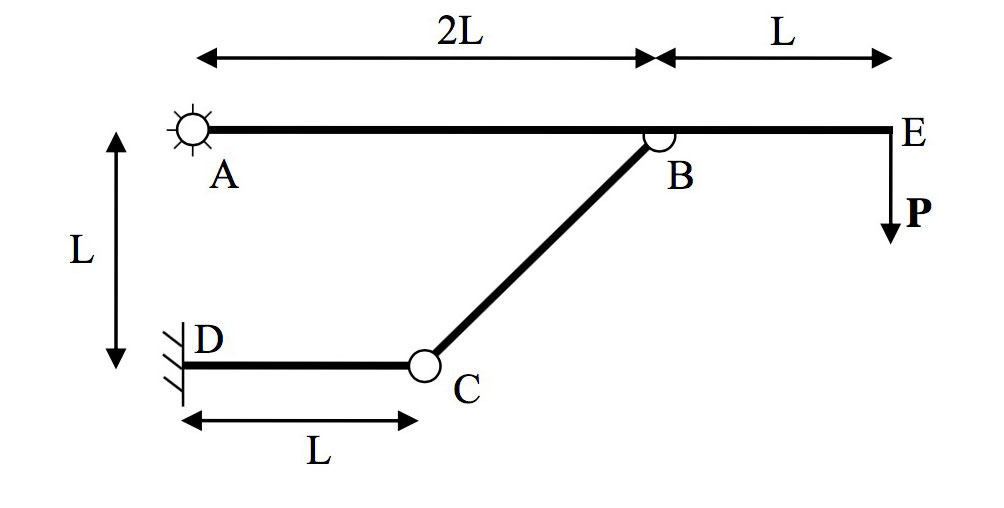
\includegraphics[width=0.75\textwidth]{2014-0407-2.jpg}
\end{figure}

La struttura in figura è soggetta al solo carico verticale P. Si chiede di calcolare:

\begin{enumerate}
\item Le reazioni vincolari in A e D.
\item Le azioni interne nell’asta AE.
\end{enumerate}

\clearpage

\subsection{Soluzione secondo esercizio}

\subsubsection{Osservazioni}

\begin{enumerate}
\item La struttura è composta da 2 aste e 3 vincoli: un incastro, una cerniera esterna ed un pendolo (o biella).
\end{enumerate}

\subsubsection{Analisi preliminare di isostaticità}
Verifico che $gdl_{tot} = gdv_{tot}$:
\begin{figure}[H]
  \begin{subfigure}[b]{.5\textwidth}
  \centering
  \[
  	gdv: \begin{cases}
		gdv_{cerniera_{esterna}} = 2\\
		gdv_{incastro} = 3\\
		gdv_{biella} = 1
  	\end{cases}
  \]
  \caption{Gradi di vincolo del sistema.}
  \end{subfigure}
  \hfill
  \begin{subfigure}[b]{.5\textwidth}
  \centering
  \[
  	gdl: \begin{cases}
  		gdl_{aste} = 6\\
  	\end{cases}
  \]
  \caption{Gradi di libertà del sistema.}
  \end{subfigure}
  \caption{Verifica preliminare di isostaticità.}
\end{figure}

\subsubsection{Primo punto}

\paragraph{Analisi dei vincoli esterni}

\begin{figure}[H]
\centering
\resizebox{.5\textwidth}{!}{% First image 2015 06 29

\begin{tikzpicture}

  \tiny


  \point{c}{0}{0}
  \point{c1}{0}{0.8}
  \point{c2}{-0.8}{0}
  \point{a}{2-1.41421}{1.41421}
  \point{a1}{2-1.41421}{0.8+1.41421}
  \point{d}{2}{0}
  \point{b}{2+1.41421}{-1.41421}
  \point{b1}{2+1.41421}{-1.41421-1.3}

  \beam{2}{c}{d}[0][1];
  \beam{2}{a}{b};

  \load{1}{a}[180][0.5]
  \load{1}{a1}[270][0.5]

  \load{2}{c}
  \load{1}{c}[180][0.5]
  \load{1}{c}[270][0.5]

  \load{1}{b1}[90][1]

  \notation{1}{c}{$\vec{M}_C$}[below right]
  \notation{1}{c}{$\vec{H}_C$}[below left]
  \notation{1}{c}{$\vec{V}_C$}[above right]

  \notation{1}{a}{$\vec{H}_A$}[below left]
  \notation{1}{a}{$\vec{V}_A$}[above right]

  \notation{1}{b}{$\vec{F}$}[below right]

  % \notation{1}{a1}{$\vec{H}_A$}
  % % \notation{1}{d1}{$\vec{R}_D$}
  % % \notation{1}{b1}{$\vec{H}_B$}[below left]
  % \notation{1}{c1}{$\vec{F}$}[above left]

  %  % \support{3}{o};

  %  % %Degrees
  %  % \notation{1}{o}{$\alpha$}[above];
  %  % \notation{1}{a}{$\beta$}[above];

  %  % \notation{5}{o}{a}[$a$];
  %  % \notation{5}{a}{b}[$b$];
  %  % \notation{5}{o}{b}[$c$];

\end{tikzpicture}}
\caption{Analisi dei vincoli esterni}
\end{figure}

\[
\begin{cases}
	H_A = - H_D\\
	V_A + V_D = P\\
	M_D + LH_A + 3LP = 0
\end{cases}
\]

\paragraph{Analisi delle reazioni vincolari in DC}
La biella trasmette unicamente la reazione assiale, che è inclinata di $45\deg$. Le componenti cartesiane di questa reazione assiale sono quindi uguali: $R_{C_x} = R_{C_y}$.

\begin{figure}[H]
\centering
\resizebox{.5\textwidth}{!}{% First image 2015 06 29

\begin{tikzpicture}

  \tiny


  \point{d}{0}{0}
  \point{a}{0}{2}
  \point{c}{2}{0}
  \point{b}{4}{2}
  \point{e}{6}{2}

  \beam{2}{d}{c}[0][1];
  % \beam{2}{c}{b}[0][1];
  % \beam{2}{a}{e};

  % \load{1}{e}[90]

  \load{1}{d}[270]
  \load{1}{d}[180]
  \load{2}{d}

  \load{1}{c}[0]
  \load{1}{c}[90]

  % \load{1}{a}[270]
  % \load{1}{a}[180]


  \notation{1}{d}{$\vec{M}_D$}[above]
  \notation{1}{d}{$\vec{H}_D$}[below left]
  \notation{1}{d}{$\vec{V}_D$}[below right]

  \notation{1}{c}{$\vec{R}_{C_x}$}[above left]
  \notation{1}{c}{$\vec{R}_{C_y}$}[above right]

  % \notation{1}{a}{$\vec{H}_A$}[below left]
  % \notation{1}{a}{$\vec{V}_A$}[below right]

  % \notation{1}{e}{$\vec{P}$}[above right]

\end{tikzpicture}}
\caption{Analisi delle reazioni vincolari in DC.}
\end{figure}

\[
\begin{cases}
	R_{C_x} = R_{C_y}\\
	R_{C_x} = H_D\\
	R_{C_y} = V_D\\
	V_D = H_D\\
	M_D = -LR_{C_y} = -LV_D
\end{cases}
\]

Sostituisco queste relazioni nel sistema precedente e risolvo l'ultima equazione ponendo $H_A = -H_D = -V_D$ e $M_D = -LV_D$:

\[
	(-LV_D) + L(-V_D) + 3LP = 0
\]

\[
	-LV_D - LV_D + 3LP = 0
\]

\[
	V_D = \dfrac{3}{2}P
\]

Sostituisco il valore così ottenuto nelle relazioni rimanenti ed ottengo:

\begin{figure}[H]
  \begin{subfigure}[b]{.5\textwidth}
  \centering
  \[
  	A: \begin{cases}
		H_A = - \dfrac{3}{2}P\\
		V_A = - \dfrac{1}{2}P\\
  	\end{cases}
  \]
  \caption{Reazioni vincolari in A.}
  \end{subfigure}
  \hfill
  \begin{subfigure}[b]{.5\textwidth}
  \centering
  \[
  	D: \begin{cases}
  		H_D =  \dfrac{3}{2}P\\
  		V_D =  \dfrac{3}{2}P\\
  		M_D =  -\dfrac{3L}{2}P
  	\end{cases}
  \]
  \caption{Reazioni vincolari in B.}
  \end{subfigure}
  \caption{Riassunto soluzione primo punto.}
\end{figure}

\subsubsection{Secondo punto}
Essendo l'asta posizionata orizzontalmente, l'asse normale e  tangente corrispondono rispettivamente con ascisse ed ordinate.

\[
	A: \begin{cases}
		N = - \dfrac{3}{2}P\\
		T = - \dfrac{1}{2}P\\
	\end{cases}
	\qquad
	B: \begin{cases}
		N =  \dfrac{3}{2}P\\
  		T =  \dfrac{3}{2}P\\
	\end{cases}
	\qquad
	P: \begin{cases}
		N =  0
  		T =  -P\\
	\end{cases}
\]

\paragraph{Sforzo normale baricentrico} Nel tronco di asta AB lo sforzo normale risulta positivo, poiché di \textbf{trazione}. Nel tronco di asta BE invece non avviene sforzo normale.

\begin{figure}[H]
\centering
\resizebox{.5\textwidth}{!}{% First image 2015 06 29

\begin{tikzpicture}

  \tiny


  \point{c}{0}{0}
  \point{a}{0}{1}
  \point{b}{1}{0}
  \point{d}{2}{0}

   \beam{2}{c}{d}[0][1];

  \internalforces{c}{b}{1}{1}[0][blue];

\end{tikzpicture}}
\caption{Sforzo normale nell'asta AE.}
\end{figure}

\paragraph{Taglio} Nel tronco di asta AB le forze $T_A$ ed $T_B$ impongono nel tronco una rotazione \textbf{anti-oraria}, che è quindi considerata negativa, mentre nel secondo tronco BE le forze $T_B$ e $P$ impongono una rotazione \textbf{oraria}.

\begin{figure}[H]
\centering
\resizebox{.5\textwidth}{!}{% First image 2015 06 29

\begin{tikzpicture}

  \tiny


  \point{c}{0}{0}
  \point{c1}{0}{0.8}
  \point{c2}{-0.8}{0}
  \point{a}{2-1.41421}{1.41421}
  \point{a1}{2-1.41421}{0.8+1.41421}
  \point{d}{2}{0}
  \point{d1}{2-0.8}{0}
  \point{b}{2+1.41421}{-1.41421}
  \point{b1}{2+1.41421}{-1.41421-1.3}

  \beam{2}{a}{b};

  \internalforces{a}{d}{-0.707}{-0.707}[0][blue];
  \internalforces{d}{b}{0.707}{0.707}[0][red];

\end{tikzpicture}}
\caption{Taglio nell'asta AE.}
\end{figure}

\paragraph{Momento flettente} Partendo da A, che impone un taglio $T_A$ dall'alto verso il basso, possiamo vedere che le fibre tese risultano sul lato superiore dell'asta. Il momento imposto da $T_A$ raggiunge il massimo nel punto B $M_{max} = LP$, in cui viene applicata una forza $T_B$ indirizzata in senso opposto che porta il momento a raggiungere lo zero linearmente in E.
\\
\\
Percorrendo il percorso a ritroso, partendo da E, è possibile ottenere lo stesso risultato.

\begin{figure}[H]
\centering
\resizebox{.5\textwidth}{!}{% First image 2015 06 29

\begin{tikzpicture}

  \tiny


  \point{c}{0}{0}
  \point{c1}{0}{0.8}
  \point{c2}{-0.8}{0}
  \point{a}{2-1.41421}{1.41421}
  \point{a1}{2-1.41421}{0.8+1.41421}
  \point{d}{2}{0}
  \point{d1}{2-0.8}{0}
  \point{b}{2+1.41421}{-1.41421}
  \point{b1}{2+1.41421}{-1.41421-1.3}

  \beam{2}{a}{b};

  \internalforces{a}{d}{0}{-0.707}[0][red];
  \internalforces{d}{b}{-0.707}{0}[0][red];

\end{tikzpicture}}
\caption{Momento flettente nell'asta AE.}
\end{figure}

\end{document}